\documentclass{article}
\usepackage{amsmath}
\usepackage{amssymb}
\usepackage{graphicx}
\usepackage{hyperref}
\usepackage[version=4]{mhchem}


\begin{document}
(1997 National Team) How many units are in the length of the radius of the circle which passes through points \(X, Y\) and \(Z\) ? Express your answer as a decimal rounded to the nearest tenth.\\
\centering

\includegraphics[width=\textwidth]{images/204.jpg}

Solution: 11.2 (units)\\
Draw the circumcircle of triangle \(A Y Z\).\\
Draw two diameters of the circle. Label all the line segments as shown in the figure.\\
We see that \(T M=N O=2\)\\
\(X T \times T Z=Y T \times T P \Rightarrow 8 \times 12=6 \times T P \Rightarrow T P=16\).\\
Then \(Y P=22\) and \(N P=11\).\\
Applying Pythagorean Theorem to triangle NPO:\\
\(O P^{2}=N O^{2}+N P^{2}=2^{2}+11^{1}=125\)\\
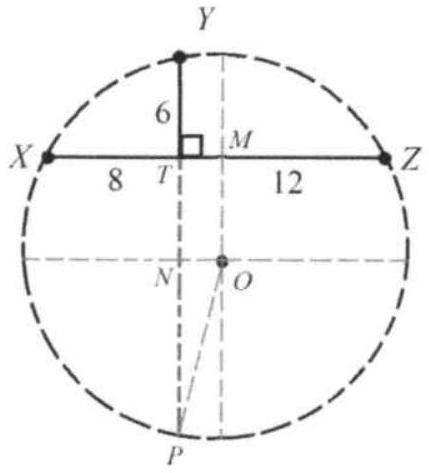
\includegraphics[width=\textwidth]{images/204(3).jpg} \(O P=\sqrt{125}=5 \sqrt{5} \approx 11.2\)


\end{document}
